\documentclass[a4paper,10pt]{article}

\usepackage[margin=2cm, tmargin=1.5in, headheight=40px]{geometry}
\usepackage[sfdefault, medium, light]{roboto}
%\usepackage[nomap]{FiraMono}
\usepackage[T1]{fontenc}
\usepackage[utf8]{inputenc}
\usepackage[spanish]{babel}
\usepackage{graphicx}
\usepackage{fancyhdr}
\usepackage{minted}
\usepackage{enumitem}
\usepackage[svgnames]{xcolor}
\setminted{style=default,bgcolor=Gainsboro}
\usepackage[allcolors={DarkSlateBlue}, colorlinks]{hyperref}

\fancyhf{}
\fancyhead[L]{
\includegraphics[height=35px]{../figuras/logoort.png}}
\fancyhead[R]{Facultad de Ingeniería \\ Cátedra de Redes y Sistemas de Comunicación}
\fancyfoot[R]{Página \thepage}
\fancyfoot[L]{Redes -- Laboratorio 4}
\renewcommand{\footrulewidth}{0.2pt}
\renewcommand{\headrulewidth}{0.2pt}

\pagestyle{fancy}


\title{\bf Redes\\Laboratorio 4 -- Capa de Red\\ Direccionamiento y ruteo estático}
\author{\bf Universidad ORT Uruguay}
\date{\bf Curso 2026}

\begin{document}

\maketitle
\thispagestyle{fancy}

En este laboratorio trabajaremos a nivel de Capa de Red, configurando de forma completa la asignación de direcciones y ruteo interno estático de una red de tipo empresarial. En particular los objetivos son:

\begin{itemize}
    \item Realizar una asignación de direcciones de una topología dada.
    \item Configurar dicha asignación en los equipos, tanto routers como hosts, de manera de implementar la capa de red.
    \item Realizar la configuración de rutas estáticas para lograr conectividad en toda la topología.
    \item Probar dicha conectividad mediante paquetes de prueba ICMP usando el comando \texttt{ping <IP destino>}.
\end{itemize}

La práctica puede realizarse de dos maneras:

\begin{enumerate}[label={\bf \alph*)}]
    \item Utilizando los equipos Cisco disponibles en el laboratorio de Redes. Dichos Routers se encuentran pre-cableados en topología de anillo, utilizando enlaces \textbf{seriales} punto a punto. Los routers disponen además de interfaces \textbf{Ethernet} (FastEthernet o GigabitEthernet, según el modelo). Sin embargo, los routers inicialmente tienen todas sus interfaces apagadas y sin configurar (tal como vienen de fábrica). Disponemos de dos anillos de 4 Routers y uno de 3 Routers, así como Switches para implementar las redes locales.
    
    En este caso, cada grupo configurará un único Router, así como los equipos conectados directamente al mismo, poniéndose de acuerdo con los restantes equipos del mismo anillo cuál es la configuración correcta de modo de que la red quede coherentemente configurada.

    \item Utilizando el simulador \href{https://www.gns3.com/}{\bf GNS3} que permite emular en una PC de escritorio una topología de red dada, creando máquinas virtuales que emulan el funcionamiento de los Routers y su sistema operativo. Se proveen en la página del curso archivos de tipo \emph{portable GNS3 project} con topologías similares a las de laboratorio. En este caso, el equipo deberá configurar \emph{toda la topología} para que quede funcionando.
    
\end{enumerate}

\section{Asignación de direcciones}

\subsection{Topología de 4 routers}

\begin{figure}
    \begin{center}
    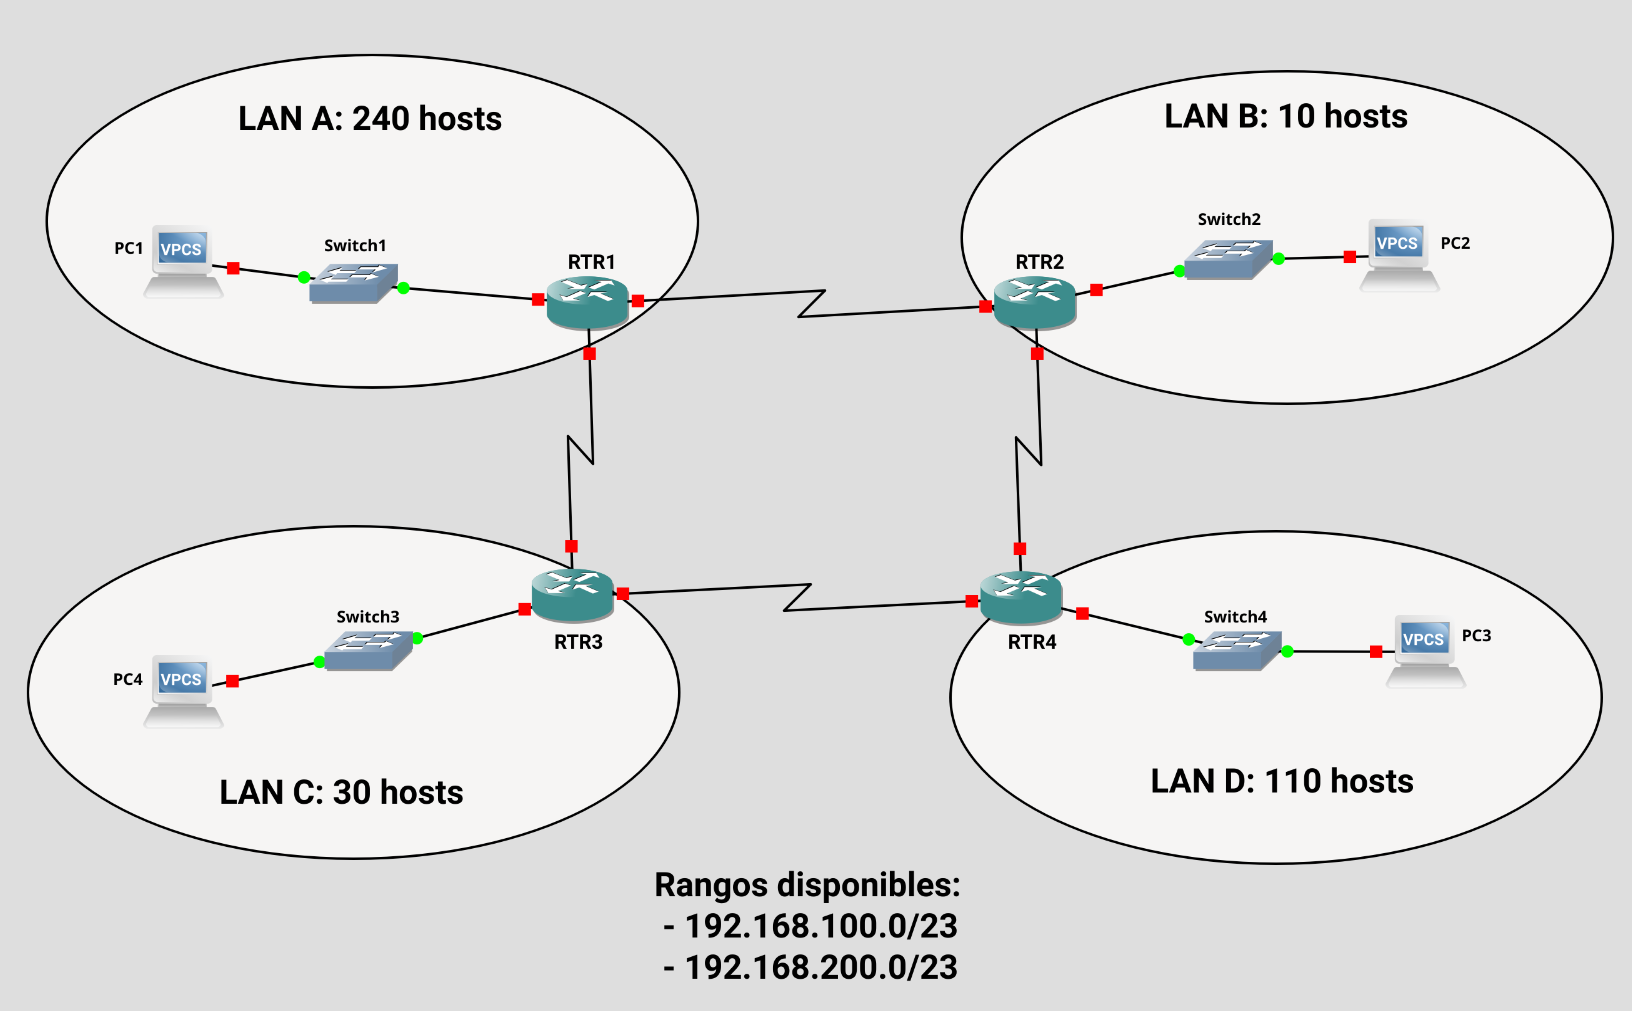
\includegraphics[width=0.95\textwidth]{../figuras/topologia_lab.png}
    \end{center}
    \caption{Topología de Red de 4 routers con rangos a asignar.}\label{fig:topologia}
\end{figure}

Realice una asignación de direcciones completa para las redes de área local de la Figura \ref{fig:topologia}, así como para los enlaces punto a punto entre routers, utilizando el rango provisto. Complete las siguientes tablas

    \begin{center}
        \bigskip
        \begin{tabular}{|p{1cm}|p{3cm}|p{3cm}|p{3cm}|p{3cm}|}
            \hline
            \textbf{Red} & \textbf{Dirección de red} & \textbf{Máscara} & \textbf{Dir. de broadcast} & \textbf{IP Router} \\ \hline
            \textbf{LAN A} & & & & \\ \hline
            \textbf{LAN B} & & & & \\ \hline
            \textbf{LAN C} & & & & \\ \hline
            \textbf{LAN D} & & & & \\ \hline
        \end{tabular}
    \end{center}

    \bigskip
    \begin{center}
        \begin{tabular}{|p{2cm}|p{2.5cm}|p{2.5cm}|p{2.6cm}|p{2.4cm}|p{2.4cm}|}
            \hline
            \textbf{Enlace} & \textbf{Dirección de red} & \textbf{Máscara} & \textbf{Dir. de broadcast} & \textbf{IP Router A} & \textbf{IP Router B} \\ \hline
            \textbf{RTRA--RTRB} & & & & & \\ \hline
            \textbf{RTRA--RTRC} & & & & & \\ \hline
            \textbf{RTRB--RTRD} & & & & & \\ \hline
            \textbf{RTRC--RTRD} & & & & & \\ \hline
        \end{tabular}
    \bigskip
    \end{center}

\subsection{Topología de 3 routers}

    Modifique ahora la asignación anterior para el caso en que hay solo 3 routers, asumiendo que la LAN D y la LAN B son una única LAN con 120 hosts.

        \begin{center}
        \bigskip
        \begin{tabular}{|p{1cm}|p{3cm}|p{3cm}|p{3cm}|p{3cm}|}
            \hline
            \textbf{Red} & \textbf{Dirección de red} & \textbf{Máscara} & \textbf{Dir. de broadcast} & \textbf{IP Router} \\ \hline
            \textbf{LAN A} & & & & \\ \hline
            \textbf{LAN B} & & & & \\ \hline
            \textbf{LAN C} & & & & \\ \hline
        \end{tabular}
    \end{center}

    \bigskip
    \begin{center}
        \begin{tabular}{|p{2cm}|p{2.5cm}|p{2.5cm}|p{2.6cm}|p{2.4cm}|p{2.4cm}|}
            \hline
            \textbf{Enlace} & \textbf{Dirección de red} & \textbf{Máscara} & \textbf{Dir. de broadcast} & \textbf{IP Router A} & \textbf{IP Router B} \\ \hline
            \textbf{RTRA--RTRB} & & & & & \\ \hline
            \textbf{RTRA--RTRC} & & & & & \\ \hline
            \textbf{RTRB--RTRC} & & & & & \\ \hline
        \end{tabular}
    \bigskip
    \end{center}


\textbf{Nota:} antes de continuar, si está trabajando con los equipos del laboratorio, comparta la asignación realizada con el resto de los grupos de su topología de modo de llegar a una asignación coherente. Compare en particular \textbf{cuál es su número de router y cuáles son sus interfaces} con el \textbf{esquema de conexión} disponible en el rack del laboratorio.


\section{Acceso a la consola de configuración}

Para conectarse a los routers, debe accederse a los mismos mediante su \emph{consola de configuración}. Típicamente esto se realiza mediante un cable dedicado y una conexión serial, que permite comunicarse con el sistema operativo del Router.

\begin{enumerate}[label={\bf \alph*)}]
\item En el caso de los equipos de laboratorio, para simplificar este proceso, se dispone de un equipo Cisco remotizador de consolas. Para acceder al Router RTRX, se debe ingresar via \texttt{telnet} al remotizador, y luego acceder a la consola del Router deseado mediante:
\begin{minted}{batch}
> telnet 172.20.20.24
> Login: grupoX
> Password: ort
\end{minted}
donde X es el no. de router.

\item En el caso de \textbf{GNS3}, luego de importar el proyecto portable, aparecen toda la topología ya conectada, incluyendo Routers y PC virtuales. En este caso se debe:
 \begin{enumerate}[label=\arabic*.]
    \item Iniciar la simulación de los equipos (ícono de Play).
    \item Hacer click-derecho y abrir una consola al equipo que se desea configurar.
 \end{enumerate}
\end{enumerate}

\section{Configuración de interfaces de los routers}

\begin{enumerate}
    \item Configure las interfaces del Router siguiendo la asignación elegida. \textbf{Tenga presente el nombre exacto} de las interfaces que los conectan con Routers vecinos. Puede ayudarse de los comandos en el apéndice.
    \item Verifique el estado de las interfaces mediante el comando \texttt{show ip interface brief}.
    \item Verifique el estado inicial de la tabla de rutas mediante el comando \texttt{show ip route}.
    \item Verifique conectividad a los routers directamente conectados mediante el comando \texttt{ping <IP>}.
\end{enumerate}

\section{Conexión de máquinas de usuario}

\begin{enumerate}
    \item Implemente la red local conectando un Switch a la interfaz Ethernet del router. Verifique que ahora la misma queda activa.
    \item Si está trabajando en el laboratorio, conecte su máquina del laboratorio a dicha red mediante un patch-cord adecuado, utilizando la tarjeta de red secundaria de la máquina.
    \item Configure la dirección IP, máscara y puerta de enlace predeterminada de su máquina para que quede conectada a la LAN adecuada.
    \item Chequee conectividad con el Router mediante \texttt{ping}. ¿Puede llegar más allá?
\end{enumerate}

\section{Implementación de rutas estáticas}

\begin{enumerate}
    \item Configure las rutas estáticas adecuadas en un router para que toda la red sea alcanzable.
    \item Si se configura un Router, pero los vecinos aún no, ¿enviar un \texttt{ping} entre dos hosts será posible? ¿Por qué?
    \item Una vez configurada toda la topología, verifique conectividad a toda la red.
\end{enumerate}


\appendix

\section{Comandos Cisco}

\begin{itemize}
    \item Ingresar al modo administrador:
\mintinline{batch}{RTRX> enable}
    \item Mostrar la configuración actual:
    \mintinline{batch}{RTRX# show running-config}
    \item Mostrar las interfaces (resumen): \mintinline{batch}{RTRX# show ip interface brief}
    \item Mostrar la tabla de rutas:
    \mintinline{batch}{RTRX# show ip route}
    \item Entrar al modo configuración: \mintinline{batch}{RTRX# configure terminal}
    \item Entrar a la conf. de interfaz (ej: FastEthernet 0/0): \mintinline{batch}{RTRX(config)# interface FastEthernet 0/0}
    \item Asignar IP a una interfaz: \mintinline{batch}{RTRX(config-if)# ip address <IP> <mascara>}
    
    donde la IP y la máscara van en formato decimal separadas por puntos.
    \item Encender una interfaz: \mintinline{batch}{RTRX(config-if)# no shutdown}
    \item Asignar IP de broadcast: \mintinline{batch}{RTRX(config-if)# ip broadcast-address <IP>}
    \item Crear una ruta estática: \mintinline{batch}{RTRX(config)# ip route <dir. Red> <máscara> <nextHop>}
    \item Salir de un submenú: \mintinline{batch}{RTRX(config)# exit}
    \item Realizar un \texttt{ping}: \mintinline{batch}{RTRX# ping <IP_destino>}
\end{itemize}

\section{Comandos GNS3 virtual PCs}

\begin{itemize}
    \item Configurar la IP de una PC:
\mintinline{batch}{PC_X> ip <direccion> <mascara> <ruta_por_defecto>}
    \item Mostrar la configuración actual:
    \mintinline{batch}{PC_X> show ip}
    \item Realizar un \texttt{ping}: \mintinline{batch}{PC_X> ping <IP_destino>}
\end{itemize}

\end{document}